%
% vim:set expandtab tabstop=4 shiftwidth=4:
%


This tutorial provides a brief introduction to the main features of
openBliSSART. First, we will describe basic source separation that results in
an audio file for each component. Second, we will move towards supervised
component classification using a data set, separating audio files into signals
corresponding to classes, like music and speech.


\section{Basic Source Separation}

In this section, we will explain the basic steps needed for non-negative matrix factorization (NMF)-based source separation. You will need some music files, preferably short segments ($\approx$ 10\,s) in WAV format. A good choice is to use the WAV files from the {\tt demo/wav} directory in the openBliSSART source distribution, for example. Upon completion of this section, you will be able to extract and listen to the components generated by NMF, and synthesize WAV files for them.

In the first step, we will use the ``Browser'' GUI application
which can be found in the {\tt bin} directory of the openBliSSART installation
tree.

Upon starting the browser, you will notice a tree view on the left hand side
which at the first start contains only four entries (nodes), namely
``Classification objects'', ``Labels'', ``Processes'' and ``Responses''. 
For the purpose of this section, only the ``Classification objects'' will be relevant.

The right hand side of the browser window is used to display and edit the
objects you have selected in the tree view.


\subsection{Separation with the Browser}

Probably the easiest way to use NMF is via the ``Import audio'' dialog of the Browser which can be accessed using the corresponding button on the bottom of the left side panel.

\begin{figure}
    \centering
    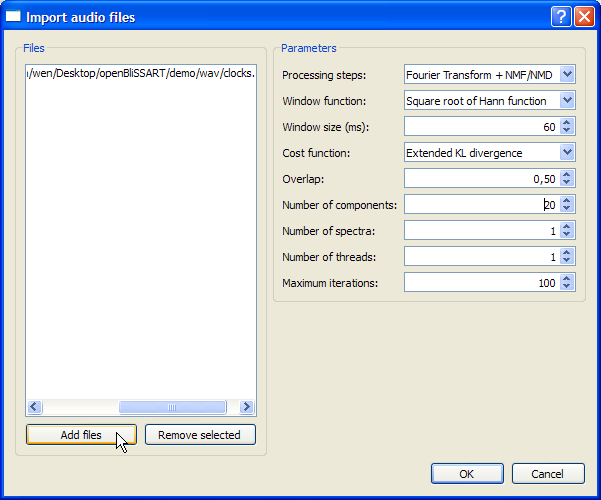
\includegraphics[width=\textwidth]{tutorial-media/ImportAudio1.png}
    \caption{%
        \label{figure:TutorialImportAudio1}%
        ``Import audio'' dialog
    }
\end{figure}

\noindent Click ``Add files'', then select an audio file from the {\tt demo/wav} folder of the openBliSSART source distribution.
For once, use the parameters as shown in
Figure~\ref{figure:TutorialImportAudio1}. A progress window as shown in
Figure~\ref{figure:TutorialBrowserPlayback} should appear. The separation
process can take several seconds, depending on your hardware.

\begin{figure}
    \centering
    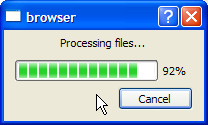
\includegraphics[width=.4\textwidth]{tutorial-media/BrowserImportProgress.png}
    \caption{%
        \label{figure:TutorialBrowserImportProgress}%
        Progress display when importing audio
    }
\end{figure}

\noindent Once the separation process has finished, several items under the
``Classification objects'' node in the browser tree view should have been
generated. Click one of them, and it will be synthesized into an audio signal
which you can play back using the buttons in the right part of the window.

\begin{figure}
    \centering
    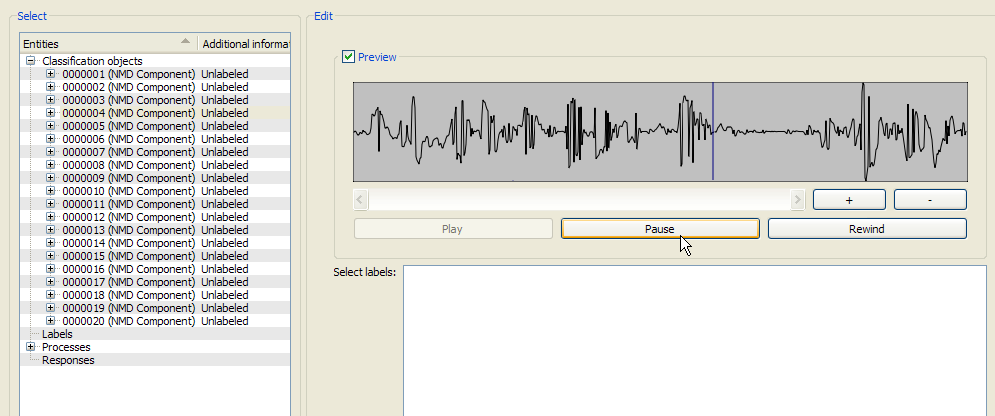
\includegraphics[width=\textwidth]{tutorial-media/BrowserPlayback.png}
    \caption{%
        \label{figure:TutorialBrowserPlayback}%
        Component playback in the browser
    }
\end{figure}

\noindent You can also export the components as audio signals in the WAV
format. To this end, select all of the components (click the first, then
Shift-click the last), right-click, and a context menu as in
Figure~\ref{figure:TutorialExportAsWav} will appear.

\begin{figure}
    \centering
    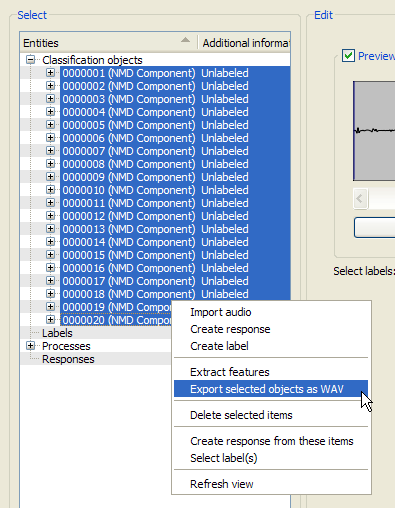
\includegraphics[width=.6\textwidth]{tutorial-media/ExportAsWav.png}
    \caption{%
        \label{figure:TutorialExportAsWav}%
        Exporting components as WAV files
    }
\end{figure}

Select the ``Export selected objects as WAV'' item, and in the appearing dialog
choose a directory where you want to create the WAV files.

The next step of this tutorial will show how you can mix these components together using the free audio editor Audacity, and manually subtract some components. You can skip this part if you do not have, and do not want to install Audacity, and move to the ``Command line separation'' section below.

\subsection{Manual Component Mixing}

Start Audacity, and select ``Import audio'' from the ``Project'' menu. Select all of the WAV files that you exported from the Browser in the previous step. The 20 components should appear as signals below each other in the Audacity window, as shown in Figure~\ref{figure:TutorialAudacityMix}.

\begin{figure}
    \centering
    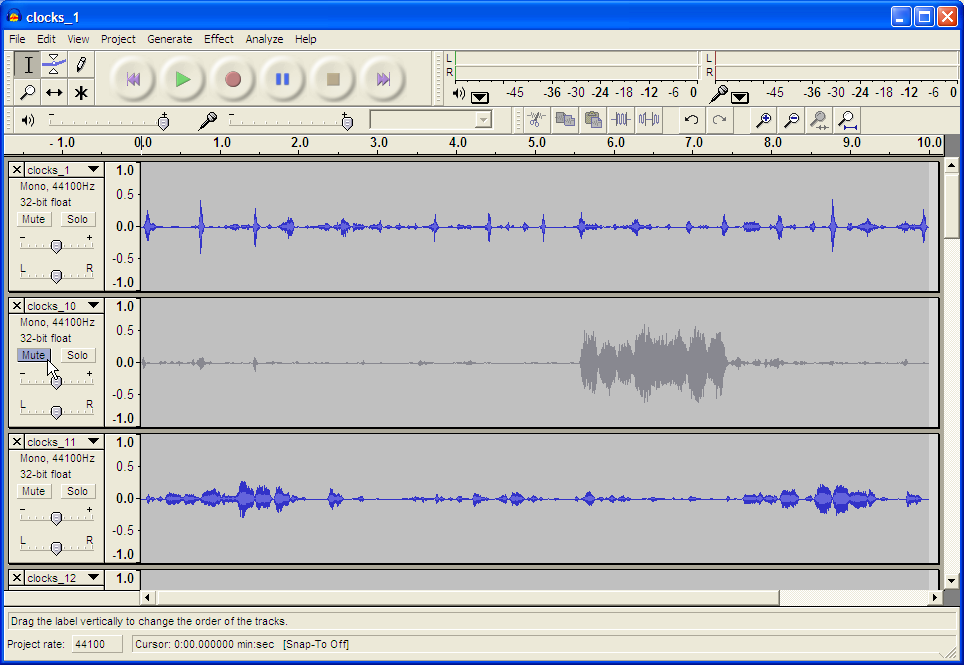
\includegraphics[width=\textwidth]{tutorial-media/AudacityMix.png}
    \caption{%
        \label{figure:TutorialAudacityMix}%
        Mixing components in Audacity
    }
\end{figure}

First, listen to the mix of all components. Depending on the type of music,
there are probably hearable artefacts, resulting from the information reduction
performed by NMF for separation.

By using the ``Mute'' and ``Solo'' buttons, you can mute some of the
components, or mute all other components, respectively. Try to identify
components which represent drum sounds using the ``Solo'' button. Normally,
this is quite easy as they show a high degree of periodicity. Now mute the
identified drum components, and listen to the result.


\subsection{Command Line Separation}

\noindent An alternative to the browser is the {\tt septool} (Separation Tool) command line
application, which is more flexible, and has more separation features than the
browser. The separation process that you performed using the ``Import audio''
dialog can be realized with {\tt septool} as follows. Open a command line window, change to the {\tt bin} directory within the openBliSSART installation directory, and type 

\begin{verbatim}
septool <file.wav>
\end{verbatim}

The default options correspond to the parameters shown in Figure~\ref{figure:TutorialImportAudio1}. After executing this command, open the browser again. There should now be 40 Classification Objects listed (20 from the recent {\tt septool} process, and 20 from the previous separation using the browser). Note that if you left the browser open while running the {\tt septool}, you have to refresh the view using the F5 key.

The {\tt septool} also has the feature to directly save the separated components as WAV files. Open a command line window, change to the openBliSSART installation directory, and type

\begin{verbatim}
septool -v -p <file.wav>
\end{verbatim}

The {\tt -v} option tells the tool not to write to the database (hence the
components will not be visible in the browser), and the {\tt -p} option causes
the components to be exported as WAV files. Change to the directory where your
input WAV file resides. There should now be files named {\tt file\_00.wav},
\dots, {\tt file\_19.wav} corresponding to the 20 components. You can use them
for the mixing process as described above.

As an exercise, you can repeat the separation and mixing procedure using
different parameters. For once, try the ``Squared Euclidean distance'' cost
function that is available in the ``Import audio dialog'' (instead of the
default ``Extended KL divergence''). You can also choose other values for
window size, overlap, window function, etc. 

The above {\tt septool} command can be adjusted to select squared Euclidean
distance as cost function, and to use a window size of 40\,ms with the
following options:

\begin{verbatim}
septool --cost-function=ed -s40 -v -p <file.wav>
\end{verbatim}

You can also try different numbers of components (in the ``Input audio'' dialog
of the browser as well using the {\tt -c<number>} option of the {\tt septool}).

\noindent {\bf Congratulations, you have finished the first part of openBliSSART's tutorial!}


\section{Supervised Component Classification}
\label{sec:SupervisedCC}

In this section, we will consider supervised component classification. This is
basically the procedure you did above, but instead of manually mixing the
tracks, a classifier is used that assigns each component automatically.  This
is exactly what the openBliSSART demonstrator for drum beat separation does --
check it out (in the {\tt demo} subdirectory of the openBliSSART distribution)
if you have not yet done so!
 
In this tutorial, instead of drum beat separation, we will now use the scenario
of speech and music discrimination, assuming that you have recordings available
that correspond to each of these classes.

In the first step, we will create a data set containing components from speech
and music signals. For this purpose, we will again use the ``Browser'' GUI.
Upon completion of this section, you will know what the background of the
``Labels'' and ``Responses'' is, and where ``Classification objects'' got their
name. 


\subsection{Importing Audio Files}

To start with, we will now import audio files and separate them into components
using NMF.

Simply click the ``Import audio'' button in the lower left corner of the browser
window so that the corresponding ``Import audio'' dialog (figure
\ref{figure:TutorialImportAudio}) appears.

\begin{figure}
    \centering
    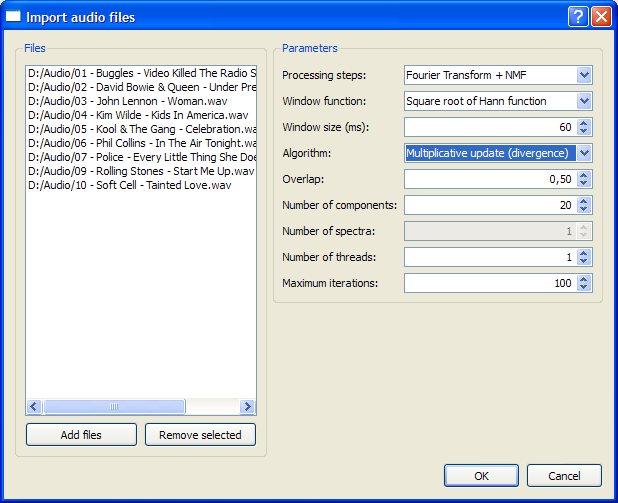
\includegraphics[width=\textwidth]{tutorial-media/ImportAudio.png}
    \caption{%
        \label{figure:TutorialImportAudio}%
        ``Import audio'' dialog
    }
\end{figure}

Ensure that the parameters on the right hand side are set exactly as in figure
\ref{figure:TutorialImportAudio} and select some audio files (WAV or MP3)
containing \emph{music}, preferably around 10-20 seconds long. Then click ``Ok''
and wait for the process to finish. Depending on the number and length of your
audio files, this process may take several minutes as it is computationally
intensive. In order to increase performance on multicore systems, you can adapt
the ``Number of threads'' settings to reflect the number of available cores
before actually starting the process.\\

Once the process has completed, you can expand the ``Classification objects''
node in the tree view so as to examine the entries reflecting the separated
components. The second column states that they are still ``Unlabeled'' --
we will take care of that in the next step.\\

However, at first please repeat the above procedure while this time selecting
audio files containing \emph{speech}. Make sure to remember how many audio files
of each class (speech and music) you have imported as this will simplify the
next step.


\subsection{Defining Classes}

Having imported the neccessary audio files, we will now define the two classes
``Speech'' and ``Music'' by creating two corresponding labels. Click the
``Create label'' button in the lower left corner of the browser window. A new
label entry will be inserted under the ``Labels'' node of the tree view with its
text defaulting to the current date and time. Use the textfield on the right
hand side to change the text to something more meaningful (like ``Music''), then
hit the ``Save'' button. Repeat this step for the ``Speech'' label. The
``Labels'' node should now look like in figure \ref{figure:TutorialLabels}.

\begin{figure}
    \centering
    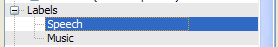
\includegraphics[width=.5\textwidth]{tutorial-media/Labels.png}
    \caption{%
        \label{figure:TutorialLabels}%
        Two defined labels
    }
\end{figure}

Next, we assign these labels to the separated components which we just have
created. Try and select a component in the tree view, and a preview as well as a
list of our labels will then appear on the right hand side (see figure
\ref{figure:TutorialClassificationObjectView}).

\begin{figure}
    \centering
    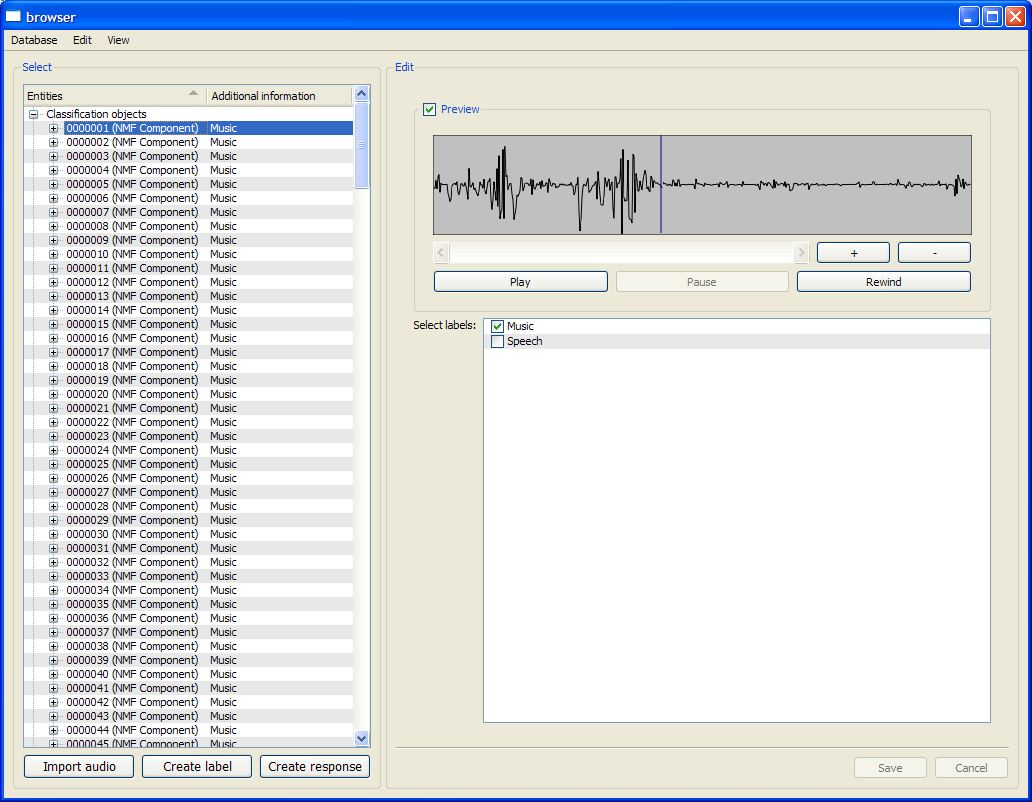
\includegraphics[width=\textwidth]{tutorial-media/ClassificationObjectView.png}
    \caption{%
        \label{figure:TutorialClassificationObjectView}%
        View of a classification object (NMF component)
    }
\end{figure}

Should you want to listen to the selected component, for example to inspect the
results of the NMF procedure, make sure that the ``Preview'' checkbox is
enabled. Once the preview is available, you can listen to the component, move
around, and zoom in and out within the respective signal data by using the
corresponding buttons inside the preview area.\\

While it is possible to assign labels to each component individually using the
checkboxes on the right hand side, for our scenario it is much more convenient
to select all components that were created from music files (remember how many
it were?), then right-click to open the context menu and use the ``Select
label(s)'' item (see figure \ref{figure:TutorialSelectLabels}).

\begin{figure}
    \centering
    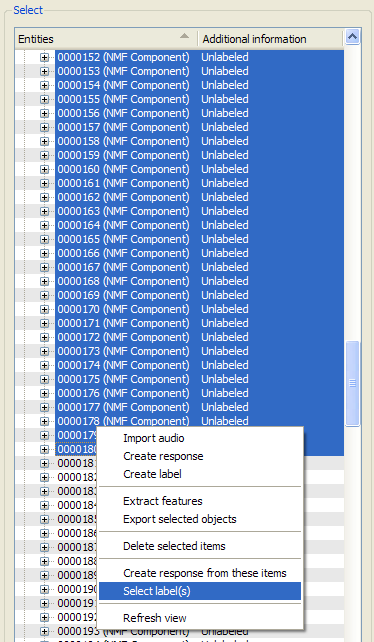
\includegraphics[width=.6\textwidth]{tutorial-media/SelectLabels.png}
    \caption{%
        \label{figure:TutorialSelectLabels}%
        Activating the context menu for components
    }
\end{figure}

A dialog will appear that allows to add one or more labels to all selected
components at the same time. Select ``Music'' and click ``Ok'', then wait for
the operation to finish. Upon completion, all selected components should show
the label ``Music'' instead of ``Unlabeled'' in the second column. By the way,
you can always refresh the tree view by either pressing F5 or selecting
``Refresh view'' from the application's ``View'' menu.\\

Repeat the above procedure for the remaining components, yet this time assign
the label ``Speech''.


\subsection{Feature Extraction}

The next step towards creating a data set is to extract features from the
created components. Again, this is very simple: Just select ``Extract features
from all data descriptors'' from the application's ``Database'' menu. Another
dialog will appear, prompting you for the number of feature extraction tasks to
start.  Remember that if you have a multicore system, you might want to set this
number to the number of cores for maximum performance, but usually feature
extraction is done quite fast anyway.\\

After the feature extraction has completed, expand one of the classification
object nodes and in turn also the ``Data descriptors'' node inside. Three
entries will appear: ``Gains'', ``Phase Matrix'' and ``Spectrum''. The phase
matrix is only used for conversion of components to wave files, features are
extracted from either one of the other two elements. Open the nodes ``Gains'' or
``Spectrum''. A list of features with values will be displayed (see figure
\ref{figure:TutorialFeatureSubtree}). The numbers inside the parentheses are
feature parameters (such as the MFCC index). The meanings of the features are
discussed in \cite{Schuller2009}.

\begin{figure}
    \centering
    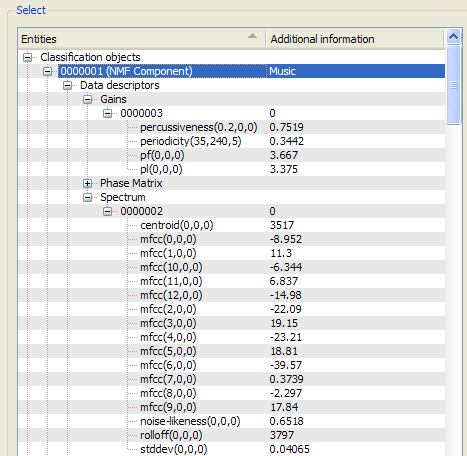
\includegraphics[width=.8\textwidth]{tutorial-media/FeatureSubtree.png}
    \caption{%
        \label{figure:TutorialFeatureSubtree}%
        Feature subtree of a classification object
    }
\end{figure}


\subsection{Defining a Response}

Eventually we will have to feed the extracted features to a support vector
machine (SVM). To this end, we create a response variable from all components we
have in the database.

Click the ``Create response'' button in the lower left corner of the browser
window. A response entry will be created under the ``Responses'' node of the
tree view. Like it was the case for labels, the name of the new response
defaults to the current date and time. Use the textfield on the right hand side
to change it into something more meaningful, like for example ``Speech
vs. music'' (see igure \ref{figure:TutorialEditResponse}).

Then click the ``Add CLOs by label'' button and select both labels (``Music''
and ``Speech'') in the corresponding dialog. After clicking ``Ok'', your
response should look like in figure \ref{figure:TutorialEditResponse}.

\begin{figure}
    \centering
    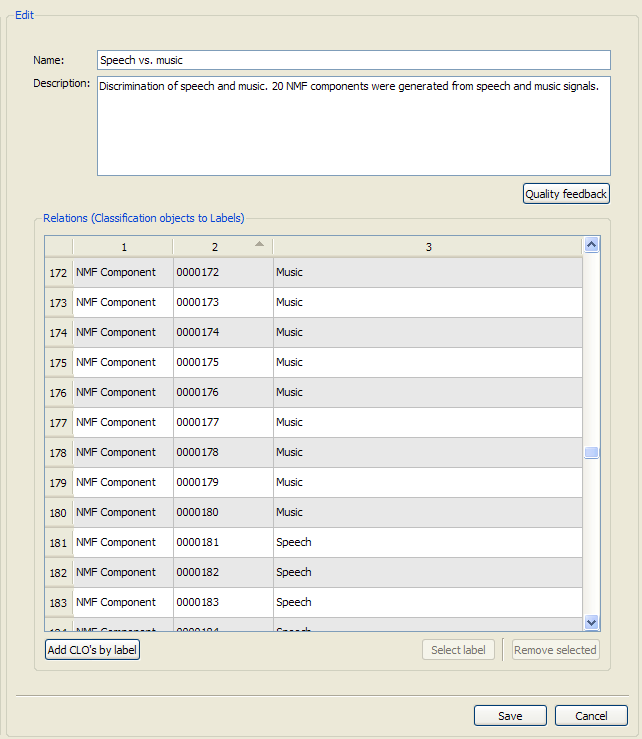
\includegraphics[width=\textwidth]{tutorial-media/EditResponse.png}
    \caption{%
        \label{figure:TutorialEditResponse}%
        Editing a response
    }
\end{figure}


\subsection{Cross-Validation}

To assess the quality of the response we have just defined, we might perform a
stratified 10-fold cross validation. Currently this function is not accessible
from the browser, but is available through a separate tool ({\tt cvtool}).

Open a shell (or Windows command prompt), change to the {\tt bin} directory of
the openBliSSART installation tree and type

\begin{verbatim}
cvtool -r1
\end{verbatim}

\noindent assuming the response has the ID\,1, which is the case if it is the first
response you created -- otherwise, check the number appearing before the
respective response's name in the tree view.\\
The cross-validation tool should output something like this:

\verbatiminput{tutorial-media/crossvalidation.txt}


\subsection{Using a Response for Blind Source Separation}

Finally, we are now able to separate audio files into their music and speech
parts by means of the response that we have created.\\

For this purpose, we also use a command-line tool ({\tt septool}). We want the
separation tool to perform NMF into 20 components using a window size of 60\,ms,
then classify the components by a support vector machine trained on the response
we have defined in the previous steps, and eventually create audio files by
summing up all components for each class and transforming them back into the
time domain, i.e. re-synthesizing the results into an appropriate number of
files depending on the number of distinct classes that the given response
uses. Thus the command line for an arbitrary input file \verb|file.wav| is as
follows:

\begin{verbatim}
septool -c20 -s60 -l1 -v file.wav
\end{verbatim}

Again, it is assumed that our response has ID\,1. The {\tt -v} (``volatile'')
option has been added here because we do not want to store additional components
from the given input file \verb|file.wav| into the database.\\

The result of this procedure will be two wave files, namely {\tt
  file\_Speech.wav} and {\tt file\_Music.wav}. Of course, you can replace {\tt
  file.wav} by any suitable WAV or MP3 file. Try mixing speech and music
together and then separating them using the separation tool like described above.\\

\noindent \textbf{Congratulations, you have just finished openBliSSART's
  introductory tutorial. For an in-depth discussion of openBliSSART's features
  and toolbox, move on to the next sections.}
